\documentclass[11pt]{article}
\usepackage[utf8]{inputenc}
\usepackage[T1]{fontenc}
\usepackage{amsmath,amssymb}
\usepackage{booktabs}
\usepackage{graphicx}
\usepackage{geometry}
\geometry{margin=1in}
\usepackage{authblk}
\usepackage[hidelinks]{hyperref}
\usepackage{xurl}
\usepackage{caption}
\usepackage{xcolor}
\usepackage{titlesec}
\usepackage{tikz}
\usepackage{enumitem}
\usepackage[section]{placeins}
\usetikzlibrary{positioning,arrows.meta}
\definecolor{navy}{HTML}{1A3A5C}
\definecolor{accent}{HTML}{2563EB}
\titleformat{\section}{\normalfont\Large\bfseries\color{navy}}{\thesection}{1em}{}
\titleformat{\subsection}{\normalfont\large\bfseries\color{accent}}{\thesubsection}{1em}{}
\graphicspath{{figures/}}
\setlength{\emergencystretch}{2em}

\newcommand{\gap}{\operatorname{gap}}
\newcommand{\repo}{\url{https://github.com/craigouma/bias-bounty-mapping-equity-challenge}}

\title{\textbf{Code Review Documentation: Bias Bounty Mapping Equity
Challenge, Submission S25}}

\author[1]{Craig Carlos Ouma\thanks{%
Correspondence: \texttt{craigcarlos95@gmail.com}. Zindi:
\texttt{craigouma}. Reviewed submission: \texttt{2ncgdcQQ}, file
\texttt{S25\_20261030-1227-03\_model-45a6fcc.csv}. Code: \repo, tag
\texttt{code-review}.}}
\affil[1]{Independent Researcher}
\date{November 4, 2026}

\begin{document}
\maketitle

\begin{abstract}
\noindent
This document accompanies the code for submission S25 (\texttt{2ncgdcQQ})
to the Bias Bounty Mapping Equity Challenge. S25 scored 0.021520001 on the
public leaderboard and 0.019332115 on the private leaderboard. The solution
computes the transport, building and point-of-interest coverage gaps per
Census tract by comparing the Overture Maps release in the challenge package
with reference counts and lengths built from public sources, and combines
them into the composite score. Every step runs as a Kaggle script kernel
driven from the command line. The document follows Zindi's documentation
guideline: overview, architecture, extraction and transformation, model,
inference, run time, metrics, error handling and maintenance, followed by the
environment and the exact steps to reproduce the submitted file.
\end{abstract}

\section{Overview and objectives}

The challenge scores each of 9,794 Census tracts in five hazard regions with
a coverage gap between 0 (Overture matches the reference) and 1 (Overture
holds nothing the reference holds). The score is the mean of three
components that are defined for the tract: transport, building and points of
interest. No labels are provided. The objective of the code is to produce,
for every tract, the 17-column file in the format of the sample submission,
with the composite score that the leaderboard evaluates and the component
values and flags that feed the organisers' Bias Scorecard.

The solution computes each component directly from its definition. For
each tract it measures the Overture side from the challenge package and the
reference side from the public sources listed in Section~\ref{sec:extract},
applies the gap function and averages the defined components. There is no
trained model in S25 and no random draw affects its output.

\section{Architecture}

Figure~\ref{fig:arch} shows the data flow. Each box is one Kaggle script
kernel. A kernel reads its inputs from the outputs of the kernels it depends
on, which Kaggle mounts under \texttt{/kaggle/input}, and writes its outputs
to \texttt{/kaggle/working}. The laptop only edits code, runs unit tests on
synthetic data and drives Kaggle through its command line.

\begin{figure}[htbp]
\centering
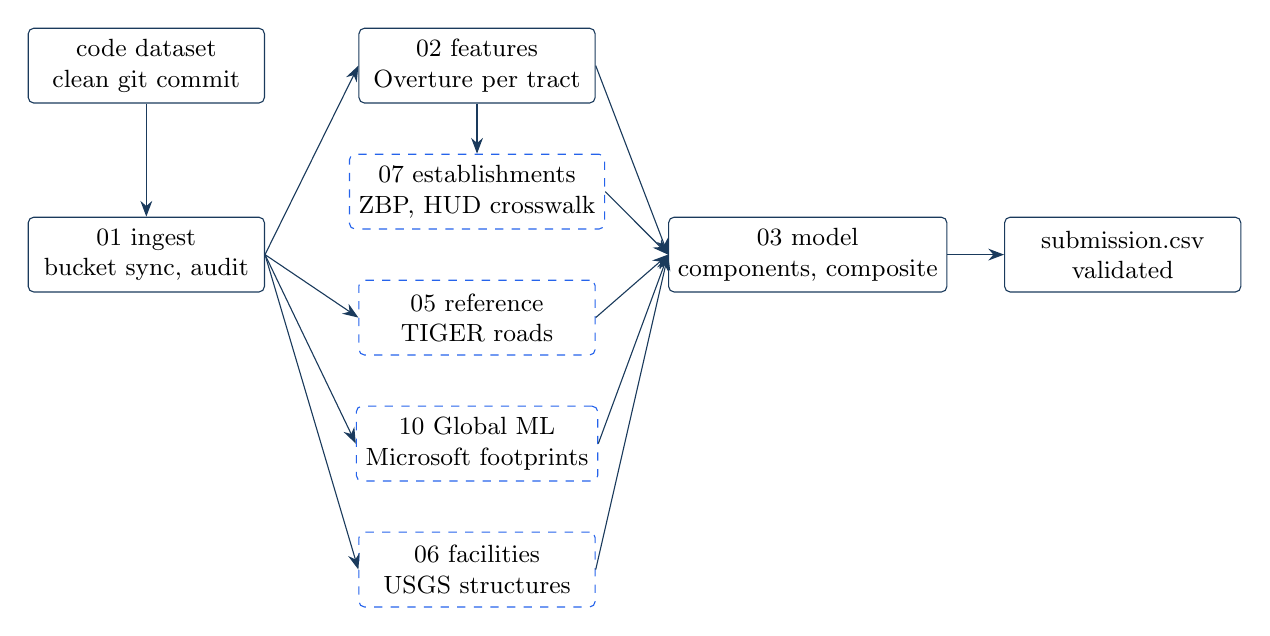
\begin{tikzpicture}[
  box/.style={draw=navy, rounded corners=2pt, align=center, font=\small,
              minimum width=3.0cm, minimum height=0.95cm},
  ext/.style={box, draw=accent, dashed},
  arr/.style={-{Stealth[length=2mm]}, draw=navy}]
\node[box] (code) at (0, 2.4) {code dataset\\clean git commit};
\node[box] (ingest) at (0, 0) {01 ingest\\bucket sync, audit};
\node[box] (feat) at (4.2, 2.4) {02 features\\Overture per tract};
\node[ext] (est) at (4.2, 0.8) {07 establishments\\ZBP, HUD crosswalk};
\node[ext] (ref) at (4.2, -0.8) {05 reference\\TIGER roads};
\node[ext] (gml) at (4.2, -2.4) {10 Global ML\\Microsoft footprints};
\node[ext] (fac) at (4.2, -4.0) {06 facilities\\USGS structures};
\node[box] (model) at (8.4, 0) {03 model\\components, composite};
\node[box] (val) at (12.4, 0) {submission.csv\\validated};
\draw[arr] (code) -- (ingest);
\foreach \n in {feat, ref, gml, fac} \draw[arr] (ingest.east) -- (\n.west);
\draw[arr] (feat) -- (est);
\foreach \n in {feat, est, ref, gml, fac} \draw[arr] (\n.east) -- (model.west);
\draw[arr] (model) -- (val);
\end{tikzpicture}
\caption{Kaggle stages on the path to S25. Solid boxes read the challenge
package only; dashed boxes also download public reference sources from their
publishers. Every stage receives the code dataset. Stage 08 (an archived
facility layer) runs as an input of stage 03 but is not read by the S25
configuration; stages 00 (environment report), 04 (analysis) and 09 (a
diagnostic) are outside the submission path.}
\label{fig:arch}
\end{figure}

\section{Extract, transform and load}

\subsection{Extract}
\label{sec:extract}

\paragraph{Challenge package.} Stage 01 lists the public Source Cooperative
bucket (\path{s3://us-west-2.opendata.source.coop/humane-intelligence/bias-bounty-mapping-equity-challenge/}) without credentials, stops
if any file name matches a denylist that includes \texttt{coverage-gap}, and
downloads 172 files (4,615,029,100 bytes): the six Overture layers of release
2026-08-19.0 per region, the ACS housing table, the per-region sample
submissions, the strata tables, the tract polygons and the boundaries. It
compares every local byte count with the bucket listing and retries a
mismatched file up to three times before failing. The challenge data are
read only from these files.

\paragraph{Public reference sources.} S25 also uses the sources in
Table~\ref{tab:sources}. Each is downloaded inside its kernel from the URL in
\texttt{configs/data.yaml} at run time, except the HUD crosswalk (see the
table note). Retrieval dates are those of the runs that produced S25; the
from-scratch rerun in Section~\ref{sec:repro} downloaded them again on 4
November 2026.

\begin{table}[htbp]
\centering
\small
\caption{Public reference sources read by S25. URLs are listed below the
table and in \texttt{configs/data.yaml}.}
\label{tab:sources}
\begin{tabular}{lllll}
\toprule
& Source & Version & Stage & Retrieved \\
\midrule
1 & Census TIGER/Line primary and secondary roads & 2025 & 05 & 27 Oct 2026 \\
2 & USGS National Map structures, state GeoPackages & 2026 & 06 & 28 Oct 2026 \\
3 & Census ZIP Code Business Patterns, totals & 2023 & 07 & 30 Oct 2026 \\
4 & HUD USPS ZIP-TRACT crosswalk$^{a}$ & Q4 2024 & 07 & 29 Oct 2026 \\
5 & Census 2020 ZCTA to tract relationship file$^{b}$ & 2020 & 07 & 30 Oct 2026 \\
6 & Microsoft Global ML Building Footprints & 2026-02-03 & 10 & 30 Oct 2026 \\
\bottomrule
\end{tabular}

\vspace{6pt}
\begin{minipage}{0.95\textwidth}\footnotesize
\begin{enumerate}[leftmargin=1.5em, itemsep=0pt]
\item \url{https://www2.census.gov/geo/tiger/TIGER2025/PRISECROADS/tl_2025_{state}_prisecroads.zip}
\item \url{https://prd-tnm.s3.amazonaws.com/StagedProducts/Struct/GPKG/STRUCT_{state}_State_GPKG.zip}
\item \url{https://www2.census.gov/programs-surveys/cbp/datasets/2023/zbp23totals.zip}
\item \url{https://www.datalumos.org/datalumos/project/219325/version/V2/view}
\item \url{https://www2.census.gov/geo/docs/maps-data/data/rel2020/zcta520/tab20_zcta520_tract20_natl.txt}
\item \url{https://minedbuildings.z5.web.core.windows.net/global-buildings/dataset-links.csv}
\end{enumerate}
\vspace{4pt}
$^{a}$ HUD serves the crosswalk only through a token API. The archived file
\path{ZIP-Tract/ZIP_TRACT_122024.xlsx} was downloaded by hand from DataLumos
project 219325, version V2, into \path{data/hud_crosswalk/}.
\path{scripts/hud_dataset.py} converts it to parquet with ZIP and tract codes
kept as text and publishes it as the Kaggle dataset
\path{<user>/bbme-hud-crosswalk}, which stage 07 reads. This is the only
manual step. $^{b}$ Downloaded by stage 07 for alternative apportionments (by
area, population and Overture places); S25 uses the HUD business-address
apportionment only.
\end{minipage}
\end{table}

\subsection{Transform}

\begin{description}[leftmargin=0pt, itemsep=4pt]
\item[Stage 02, features.] One row per scored tract. Overture road segments
of class motorway, trunk, primary and secondary are clipped to each tract
polygon and measured in geodesic metres. Overture footprints are counted by
centroid in tract. Overture places are counted per tract in total and by
\texttt{categories.primary} group (fire department, school types) following
the bucket README. Region comes from the \texttt{region} column of the sample
submission.
\item[Stage 05, reference.] TIGER/Line roads with MTFCC S1100 or S1200 are
clipped to the tract polygons and measured the same way. A road on a shared
tract boundary intersects both tracts and is counted in each.
\item[Stage 06, facilities.] USGS structure points with FCODE 74026 (fire
stations) and 73002 to 73005 (schools) are counted per tract by point in
polygon.
\item[Stage 07, establishments.] ZIP Business Patterns 2023 establishment
counts are multiplied by the HUD \texttt{BUS\_RATIO} of each ZIP and tract
pair and summed per tract.
\item[Stage 10, Global ML.] The quadkey files covering each region are read
from the index, and footprints are counted per tract by centroid.
\end{description}

Spatial work uses DuckDB 1.5.4 with its spatial extension. Two of its
behaviours fail silently and are guarded in code and tests: transforming from
EPSG:4326 without \texttt{always\_xy} returns infinite coordinates, and
\texttt{ST\_Length\_Spheroid} in longitude and latitude order returns NaN.
Every length passes through a helper in \texttt{src/bbme/db.py} that flips
coordinates and asserts a finite result, and a unit test checks it against
\texttt{pyproj.Geod} to within 0.1\,\%. GEOID is read as 11-character text
everywhere, because an integer cast drops the leading zero of Arizona's
state code.

\subsection{Load}

Each stage writes parquet tables keyed by GEOID and a manifest file to
\texttt{/kaggle/working}. Kaggle keeps these outputs as a new version of the
kernel. A downstream kernel finds its inputs by searching
\texttt{/kaggle/input} for the upstream manifest name
(\path{FEATURES_MANIFEST.json}, \path{REFERENCE_MANIFEST.json},
\path{FACILITY_MANIFEST.json}, \path{ESTABLISHMENT_MANIFEST.json},
\path{GLOBALML_MANIFEST.json}), so the code does not depend on Kaggle's
mount paths. Stage 03 joins every table on GEOID with a one-to-one check.

\section{Data model}

For an Overture quantity $O$ and a reference quantity $R$ in the same tract,
\begin{equation}
\gap(O, R) = \max\!\left(0,\; 1 - \frac{O}{R}\right), \qquad
\text{defined only when } R > 0.
\label{eq:gap}
\end{equation}

\begin{description}[leftmargin=0pt, itemsep=4pt]
\item[Transport $T$.] $O$ is the clipped Overture length of motorway, trunk,
primary and secondary roads; $R$ is the clipped TIGER S1100 and S1200 length.
\item[Building $B$.] $O$ is the Overture footprint count and $R$ the Global
ML footprint count, both by centroid.
\item[Points of interest $P$.] The facilities half $F$ is the mean of the
defined per-type gaps for fire stations and schools (Overture places in the
category against USGS points). The establishments half $E$ compares all
Overture places with the apportioned establishment count. $P$ is the mean of
the defined halves.
\end{description}

The composite is the mean of the defined components,
\begin{equation}
y = \frac{\sum_{c \in \{T, B, P\}} \delta_c\, c}{\sum_{c} \delta_c},
\end{equation}
where $\delta_c$ is 1 when component $c$ is defined. An undefined component
is written as 0 with its flag \texttt{False}. EMS stations are left out of
the facilities half; the bucket README states that EMS rarely binds, and
adding it made the public score worse.

The configuration is \texttt{configs/model.yaml} with the overrides in
\texttt{configs/final\_A.yaml}:
\begin{center}\small
\texttt{transport.source=tiger building.source=microsoft building.count=globalml}\\
\texttt{poi.source=reference poi.reference\_types=[fire,schools] poi.establishment\_weight=bus}
\end{center} With these settings every scalar that
was ever tuned on the leaderboard during the challenge is at its neutral
value (scales and levels 1.0, shrinkage 1.0), so S25 carries no
leaderboard-tuned number. The leaderboard was used to choose between whole
methods, for example which building release and which apportionment to use.

\paragraph{Feature selection and validation.} There is no learned model, so
there is no feature selection or train and validation split. The rebuilt
transport component was checked against two facts the organisers published:
the share of tracts with an undefined component per region, which it matches
to within one percentage point in all four documented regions, and the range
of Overture to TIGER length ratios across regions (0.71 to 1.59), which it
reproduces at both ends. The methodology writeup gives the full tables.

\section{Inference}

Stage 03 is the inference step. It reads the joined table, computes the
components and the composite with vectorised pandas and numpy
(\texttt{src/bbme/model.py}), writes the 17 columns in the sample's order,
row order and \texttt{region} values (\texttt{src/bbme/submit.py}), and runs
the full submission validator before saving. New data (a later Overture
release or newer reference files) enter by changing the URLs and release
names in \texttt{configs/data.yaml} and rerunning stages 01 to 03; no
retraining is needed because nothing is trained. Every run is identified by
\texttt{YYYYMMDD-HHMM-<stage>-<commit>}, and every output folder holds the
resolved configuration, the commit hash, \texttt{pip freeze}, runtime and
peak memory.

\section{Run time}
\label{sec:runtime}

Table~\ref{tab:runtime} gives the wall time and peak memory of each stage on
Kaggle CPU sessions (4 cores, 32.9\,GB RAM), for the runs that produced S25
and for the from-scratch rerun of 4 November 2026. Wall time is measured from
push to completion and includes queueing. The full chain takes about 45
minutes when the independent stages run in parallel: stage 01, then stage 05
(the longest of the parallel group), then stage 03.

\begin{table}[htbp]
\centering
\small
\caption{Stage cost on Kaggle CPU sessions.}
\label{tab:runtime}
\begin{tabular}{lrrrr}
\toprule
& \multicolumn{2}{c}{Runs behind S25} & \multicolumn{2}{c}{Rerun, 4 Nov} \\
Stage & Wall (min) & Peak RSS (GB) & Wall (min) & Peak RSS (GB) \\
\midrule
01 ingest & 5.4 & 1.39 & 7.8 & 1.47 \\
02 features & 27.9 & 6.99 & 25.5 & 6.87 \\
05 reference & 33.9 & 3.55 & 32.5 & 3.51 \\
06 facilities & 8.7 & 0.49 & 26.8 & 0.50 \\
07 establishments & 1.2 & 0.22 & 1.1 & 0.22 \\
08 archive & 1.2 & 0.45 & 1.2 & 0.50 \\
10 Global ML & 33.8 & 2.13 & 16.1 & 2.22 \\
03 model & 1.7 & 0.56 & 1.5 & 0.56 \\
\bottomrule
\end{tabular}
\end{table}

\section{Performance metrics}

\begin{itemize}[itemsep=2pt]
\item Public leaderboard RMSE: 0.021520001. Private leaderboard RMSE:
0.019332115.
\item Path to S25 on the public leaderboard: all-zero file 0.1072; best
estimate from the challenge package alone (S16) 0.0745; transport, building,
facility and establishment references rebuilt from public sources (S19)
0.0300; establishments apportioned by HUD business-address ratios (S24)
0.0238; building reference from Global ML (S25) 0.0215.
\item Reproduction: a from-scratch rerun gives a file byte-identical to the
upload, so the largest absolute difference over every float cell is 0 and no
flag differs (Section~\ref{sec:repro}).
\item Calibration of the transport component against the organisers'
published rates and ratios, described above.
\end{itemize}

\section{Error handling and logging}

\begin{itemize}[itemsep=2pt]
\item \textbf{Stale code.} Each kernel starts with a bootstrap that finds the
code dataset under \texttt{/kaggle/input} and stops if its commit hash
differs from the one the kernel was rendered with. The code dataset is only
built from a clean git tree.
\item \textbf{Truncated downloads.} Stage 01 checks every byte count against
the bucket listing, retries up to three times and fails the stage on any
remaining mismatch.
\item \textbf{File guard.} Every reader opens files through
\texttt{src/bbme/guard.py}, which accepts only allowlisted names from
\texttt{configs/data.yaml} and always rejects names containing
\texttt{coverage-gap} or \texttt{coverage\_gap}. A unit test fails if a
module opens a file without it.
\item \textbf{Silent numeric failures.} Length and area helpers assert finite
results; GEOIDs are asserted to be 11 digits after every read; joins are
checked one to one.
\item \textbf{Output validation.} Stage 03 refuses to save a file that fails
the validator: header and column order, GEOID set, row order and
\texttt{region} values equal to the sample; finite floats in $[0, 1]$ in
plain decimal notation; flags exactly \texttt{True} or \texttt{False}; a
\texttt{False} flag with a 0 gap; consistent POI flags; at least one defined
component per row.
\item \textbf{Logs.} Kaggle keeps each kernel's log with its version. The
runner saves the log locally when a stage fails, and appends every run
(run ID, stage, commit, overrides, state, wall time, peak memory) to
\texttt{docs/experiments.md}. Every submission, with its run ID, commit,
configuration and score, is in \texttt{docs/submissions.md}.
\end{itemize}

\section{Maintenance and monitoring}

\begin{itemize}[itemsep=2pt]
\item \textbf{Tests.} \texttt{make lint test} runs ruff and 178 unit tests on
synthetic fixtures, covering GEOID handling, coordinate order, the guard, the
gap and composite rules, each feature module and the submission validator.
\item \textbf{Updating inputs.} Overture release names, bucket paths and
reference URLs live in \texttt{configs/data.yaml}. A new Overture release or
reference vintage needs a rerun of stages 01 to 03 and no code change, unless
a schema changes; the stage 01 audit records schemas and distinct values to
detect that.
\item \textbf{Scaling.} Spatial joins run one region at a time with
bounding-box pruning before exact intersection, and peak memory stays under
7\,GB. More regions add rows linearly.
\item \textbf{Dependency drift.} \texttt{requirements-kaggle.txt} pins every
package the stages import. If Kaggle updates its image, the pins restore the
versions used for S25.
\end{itemize}

\section{Environment and libraries}

\begin{itemize}[itemsep=2pt]
\item Compute: Kaggle script kernels on CPU sessions, Python 3.13.15, 4 cores,
32.9\,GB RAM, internet enabled (the account needs phone verification for
internet in kernels). No GPU is used on the S25 path.
\item Orchestration: an Intel MacBook Pro with 8\,GB RAM running macOS, the
Kaggle command-line client, \texttt{uv} and GNU Make. Local Python 3.13 with
the versions locked in \texttt{uv.lock}.
\item Libraries installed in every kernel (\path{requirements-kaggle.txt};
the same list is \path{requirements.txt} in the submitted archive): duckdb 1.5.4, geopandas 1.1.4,
matplotlib 3.10.0, numpy 2.1.3, pandas 2.3.3, pyarrow 23.0.1, pyogrio 0.13.0,
pyproj 3.7.2, PyYAML 6.0.3, shapely 2.1.2. All are open source.
\item Seed: 20261025 in \texttt{configs/model.yaml}, the only source of
randomness. The S25 computation makes no random draw.
\end{itemize}

\section{Reproducing S25}
\label{sec:repro}

The reviewer needs a Kaggle account with internet enabled in kernels, the
Kaggle command-line client authenticated on the machine, \texttt{git},
\texttt{uv} and GNU Make.

\begin{enumerate}[itemsep=3pt]
\item Clone \repo{} and check out the tag \texttt{code-review}. Run
\texttt{make setup}.
\item Put the challenge \texttt{SampleSubmission.csv} in \texttt{data/} and
the uploaded S25 file at
\path{artifacts/submissions/S25_20261030-1227-03_model-45a6fcc.csv}.
\item Set \texttt{username} in \texttt{configs/kaggle.yaml} to the reviewer's
Kaggle user name and commit the change; the code dataset is built only from
a clean tree.
\item Download \texttt{ZIP\_TRACT\_122024.xlsx} (Table~\ref{tab:sources},
note $a$) into \texttt{data/hud\_crosswalk/} and run
\path{cd scripts && uv run python hud_dataset.py}.
\item \texttt{make kaggle-code}, then \texttt{make kaggle-run STAGE=01\_ingest}.
\item Run stages \texttt{02\_features}, \texttt{05\_reference},
\texttt{06\_facilities}, \texttt{08\_archive} and \texttt{10\_globalml}
(independent of one another), then \texttt{07\_establishments}, each with
\texttt{make kaggle-run STAGE=<stage>}.
\item \texttt{make reproduce FINAL=A} runs stage 03 with
\texttt{configs/final\_A.yaml} and prints the largest absolute difference and
the number of differing flags against the uploaded file.
\end{enumerate}

Each command renders the kernel, pushes it, follows its log, waits for it to
finish and downloads its small outputs to \texttt{artifacts/kaggle/}.
\texttt{make kaggle-run} accepts \texttt{PREFIX=<text>} to run a second chain
of kernels under different names.

\paragraph{Reproduction record.} Stage 03 was rerun with the S25
configuration on 30 October 2026 (run
\texttt{20261030-1512-03\_model-8f446f4}) against the upstream outputs that
produced S25, and matched the uploaded file in every cell with a largest
difference of 0. On 4 November 2026 the whole chain was rerun from scratch
under new kernel names (\texttt{repro-bbme-*}), downloading the challenge
package and every public source again (stage 01 at commit \texttt{0f182ec},
stages 02 to 10 at \texttt{db9b78d}, stage 07 at \texttt{b11465b}, stage 03 at
\texttt{64296a6}; these commits differ only in run log entries). Every
intermediate table read by S25 (TIGER lengths, USGS facility counts,
establishment counts, Global ML counts) was identical to the one behind the
uploaded file, and the Overture feature table differed only in floating-point
summation order (at most $4 \times 10^{-9}$ m in six columns that S25 does not
read). Stage 03 (run \texttt{20261104-1651-03\_model-64296a6}) produced a file
byte-identical to the uploaded S25 file:
\begin{center}\small
SHA-256 \texttt{03678f50bac04dea7c2f03abb446deb1fba45b5f55f1a7e716f2d95dbd9ff48d}
\end{center}
The installed versions of every pinned package equalled those of the original
S25 run. The commits from \texttt{64296a6} to the tag \texttt{code-review}
change comments, documentation and logs only, which
\path{git diff 64296a6 code-review -- src kaggle configs requirements-kaggle.txt}
shows.

\section{Data insights}

Stage 04 holds the exploratory analysis: unnamed road shares by tribal
status, rurality and region, maps of the composite score, and the per-stratum
tables behind the Best Bias Discovery entry. The finding, that local streets
on federally recognised reservations are unnamed in Overture 9.5 percentage
points more often than on matched non-tribal tracts, is written up at
\url{https://craigouma.github.io/bias-bounty-mapping-equity-challenge/bias-discovery/}.

\begin{figure}[htbp]
\centering
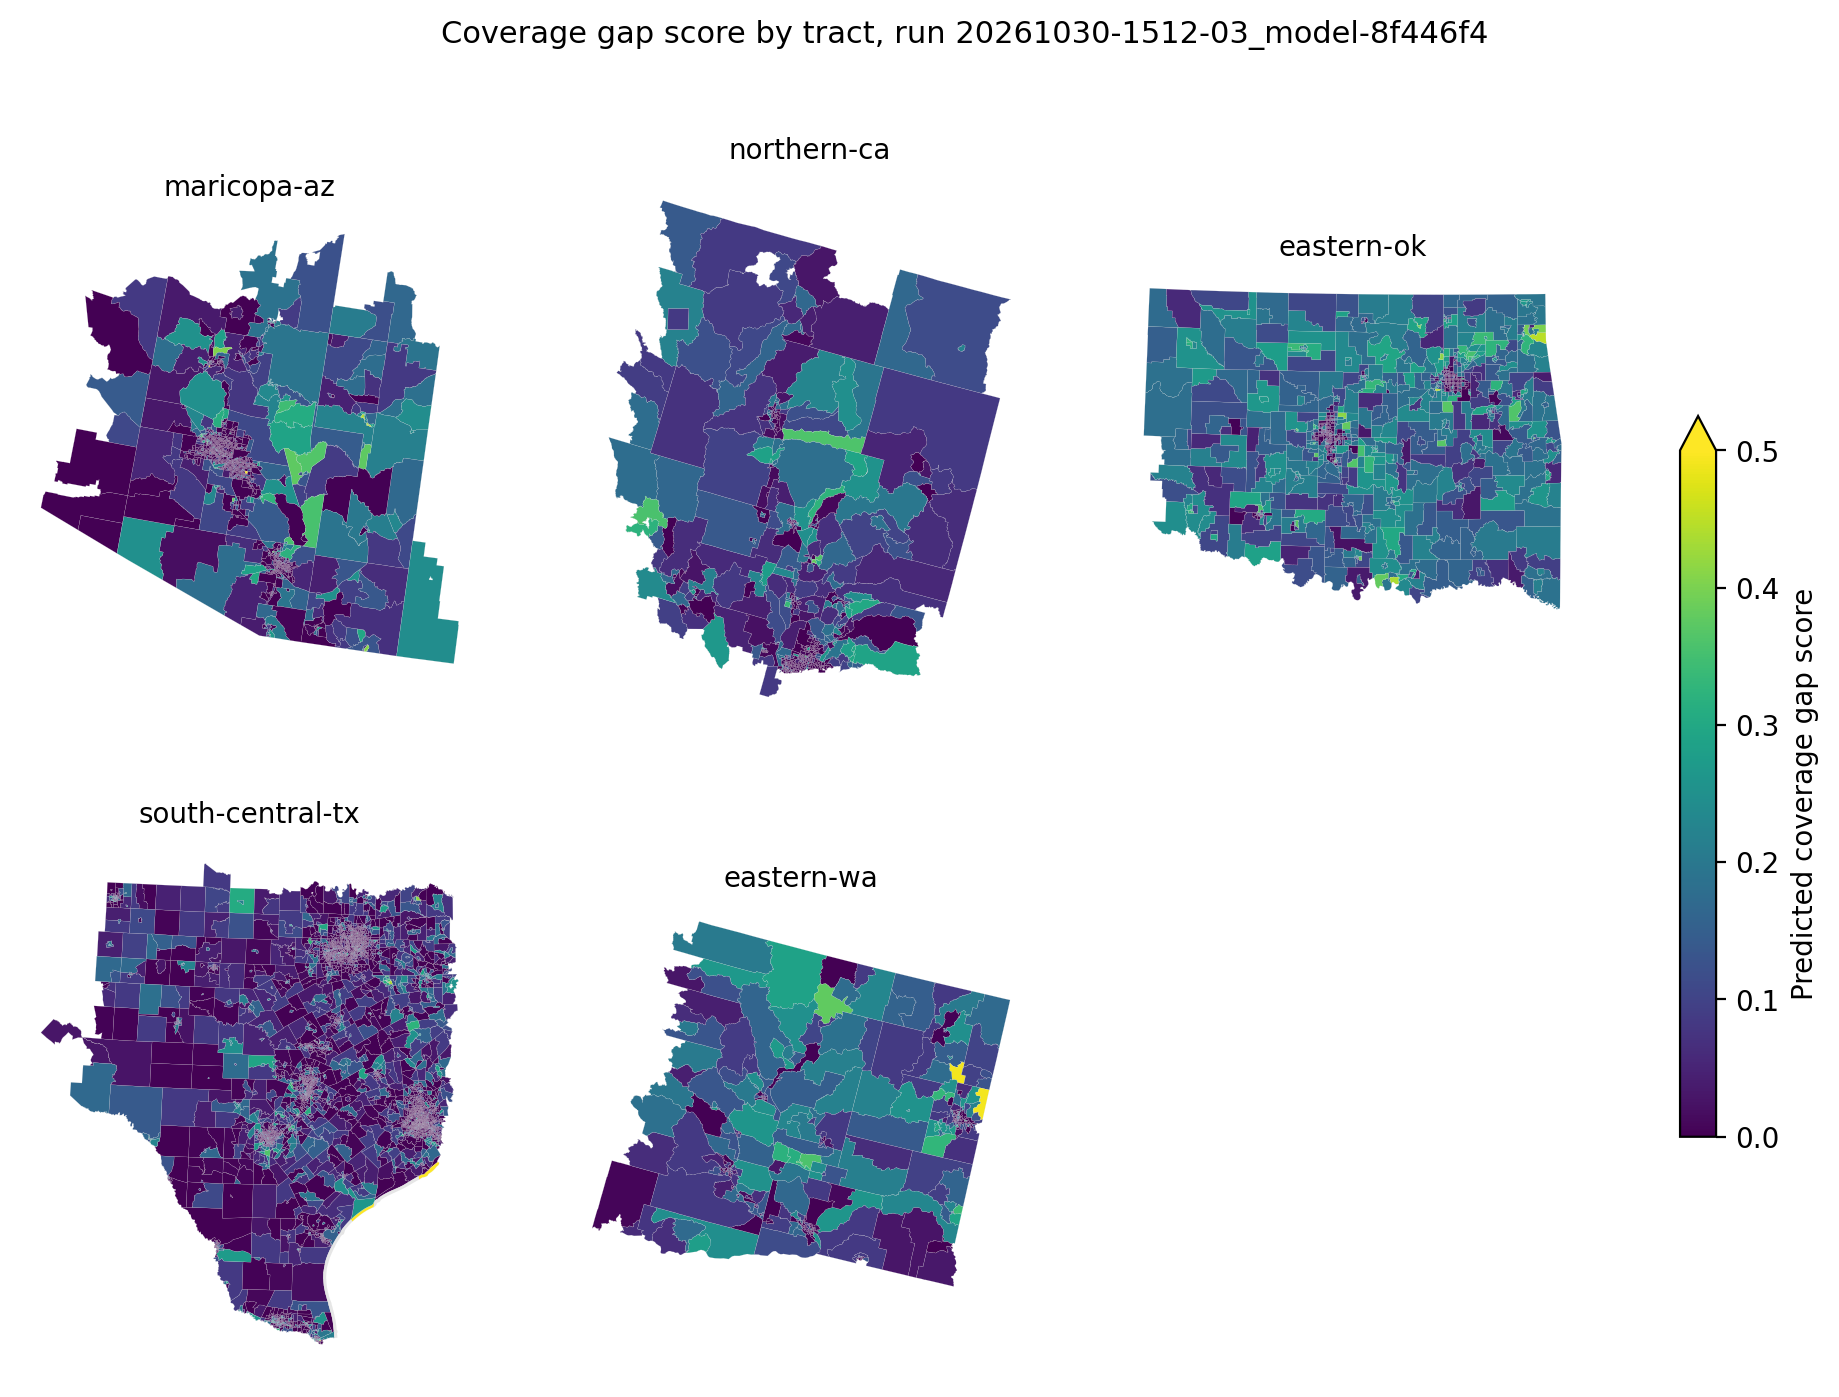
\includegraphics[width=0.9\textwidth]{fig_map_scores.png}
\caption{S25 composite coverage gap score per tract.}
\end{figure}

\end{document}
